\documentclass[10pt]{article}
% \usepackage[letterpaper,text={6.5in,8.7in},centering]{geometry}
\usepackage{curves}
\usepackage{epic,eepic,color}
%\usepackage[usenames,dvipsnames,svgnames,table]{xcolor}
% \usepackage{amssymb,amsmath,times,subfigure,graphicx,theorem}
\usepackage{alltt}
%\usepackage{warmread}
%\usepackage[all,import]{xy}
%\usepackage{eepic}
\usepackage{my_packages}
\usepackage{lastpage}
\usepackage{fancyhdr}
\pagestyle{fancy}
\cfoot{\thepage\ of \pageref{LastPage}}
\renewcommand{\headrulewidth}{0pt}
\usepackage{tikz_packages}
\renewcommand{\baselinestretch}{1.2}
\date{}

\renewcommand{\thesubsection}{\arabic{subsection}. }
\renewcommand{\thesubsubsection}{\arabic{subsection}.\arabic{subsubsection} }

\theoremstyle{definition}
\newtheorem{prob}{Problem}[section]
%\renewcommand{\theprob}{\arabic{section}.\arabic{prob}}
\renewcommand{\theprob}{\arabic{prob}}

\newenvironment{subprob}%
{\renewcommand{\theenumi}{\alph{enumi}}\renewcommand{\labelenumi}{(\theenumi)}\begin{enumerate}}%
{\end{enumerate}}%


\newcommand{\extrapage}{\clearpage\newpage\null\newpage}
%1: Choose and apply the appropriate orbital  maneuvering method to move spacecraft between orbits
%2:  Choose and apply the appropriate orbital  maneuvering method to move spacecraft between orbits
%4: Develop personal software tools to solve practical astrodynamic problems : Determine orbital parameters from ground based observations
%5: Develop personal software tools and apply orbital maneuvering
%5: Develop personal software tools and apply ground based observations

\begin{document}


\setcounter{page}{0}

\vspace*{1cm}

\centerline{\LARGE{ MAE3145: Final Exam}}
\vspace*{0.5cm}
\centerline{\Large \SI{2458052.1979}{\julianday}}%\\%\vspace*{0.5cm}

\vspace*{6cm}

\centerline{
\begin{tabular}{lll}
\hspace*{5cm}, & \hspace*{5cm}. & \hspace*{4cm}\\\hline
Last Name & First Name & Student ID
\end{tabular}}

\vspace*{6cm}

\centerline{
\begin{tabular}{|c|c|c|c|c|c|}\hline
    Prob. 1 & Prob. 2 & Prob. 3 & Prob. 4 & Prob. 5 & Total \\
    (20) & (20) & (20) & (20) & (20) & (100)\\ \hline
    \hspace*{2.2cm} & \hspace*{2.2cm} & \hspace*{2.2cm} & \hspace*{2.2cm} & \hspace*{2.2cm} & \hspace*{2.2cm} \\
                    & & & & & \\
                    & & & & & \\
\hline
\end{tabular}}

\clearpage\newpage
% \renewcommand{\theprob}{\arabic{prob} \textit{(15pt)}}

\begin{prob}
    Your spacecraft is currently in a \underline{circular} orbit about Planet X with \( \Omega = \SI{90}{\degree}\) and \( i = \SI{30}{\degree} \) relative to an inertial reference frame defined by \( \hat{x}, \hat{y}, \hat{z} \).
    At the \underline{descending node}, the following maneuver is implemented:
    \begin{align*}
        \bar \Delta v = \frac{1}{\sqrt{2}} \hat{V} - \hat{C} + \sqrt{\frac{3}{2}} \hat{N} \si{\kilo\meter\per\second} .
    \end{align*}

    Express the \( \Delta \bar v \) in terms of :
    \begin{subprob}
        \item Inertial reference frame: \( \hat x, \hat y, \hat z\)
        \item \(\norm{\Delta \bar v}, \alpha, \beta\) relative to the \( \hat V, \hat N, \hat C\) reference frame
    \end{subprob}
\end{prob}

\extrapage
\extrapage

\begin{prob}
    Assume that a spacecraft is moving in an orbit about the Earth characterized by \( e = 0.5\) and \( a = 4 R_\oplus\).
    To meet some scientific objective, an \underline{in-plane} maneuver is planned to adjust the orbit.
    The new orbit has exactly the same eccentricity and semi-major axis but periapsis will advance by \SI{90}{\degree}.
    \begin{subprob}
        \item The maneuver can be implemented at one of two values of true anomaly. 
            Determine these two options.
        \item Assume that the maneuver will be implemented at \( \theta = \SI{45}{\degree}\).
            Determine the required maneuver in terms of \( \norm{\Delta \bar v} \) and \(\alpha\).
    \end{subprob}
    \vspace*{9cm} 
    \begin{figure*}[hb]
        \centering
        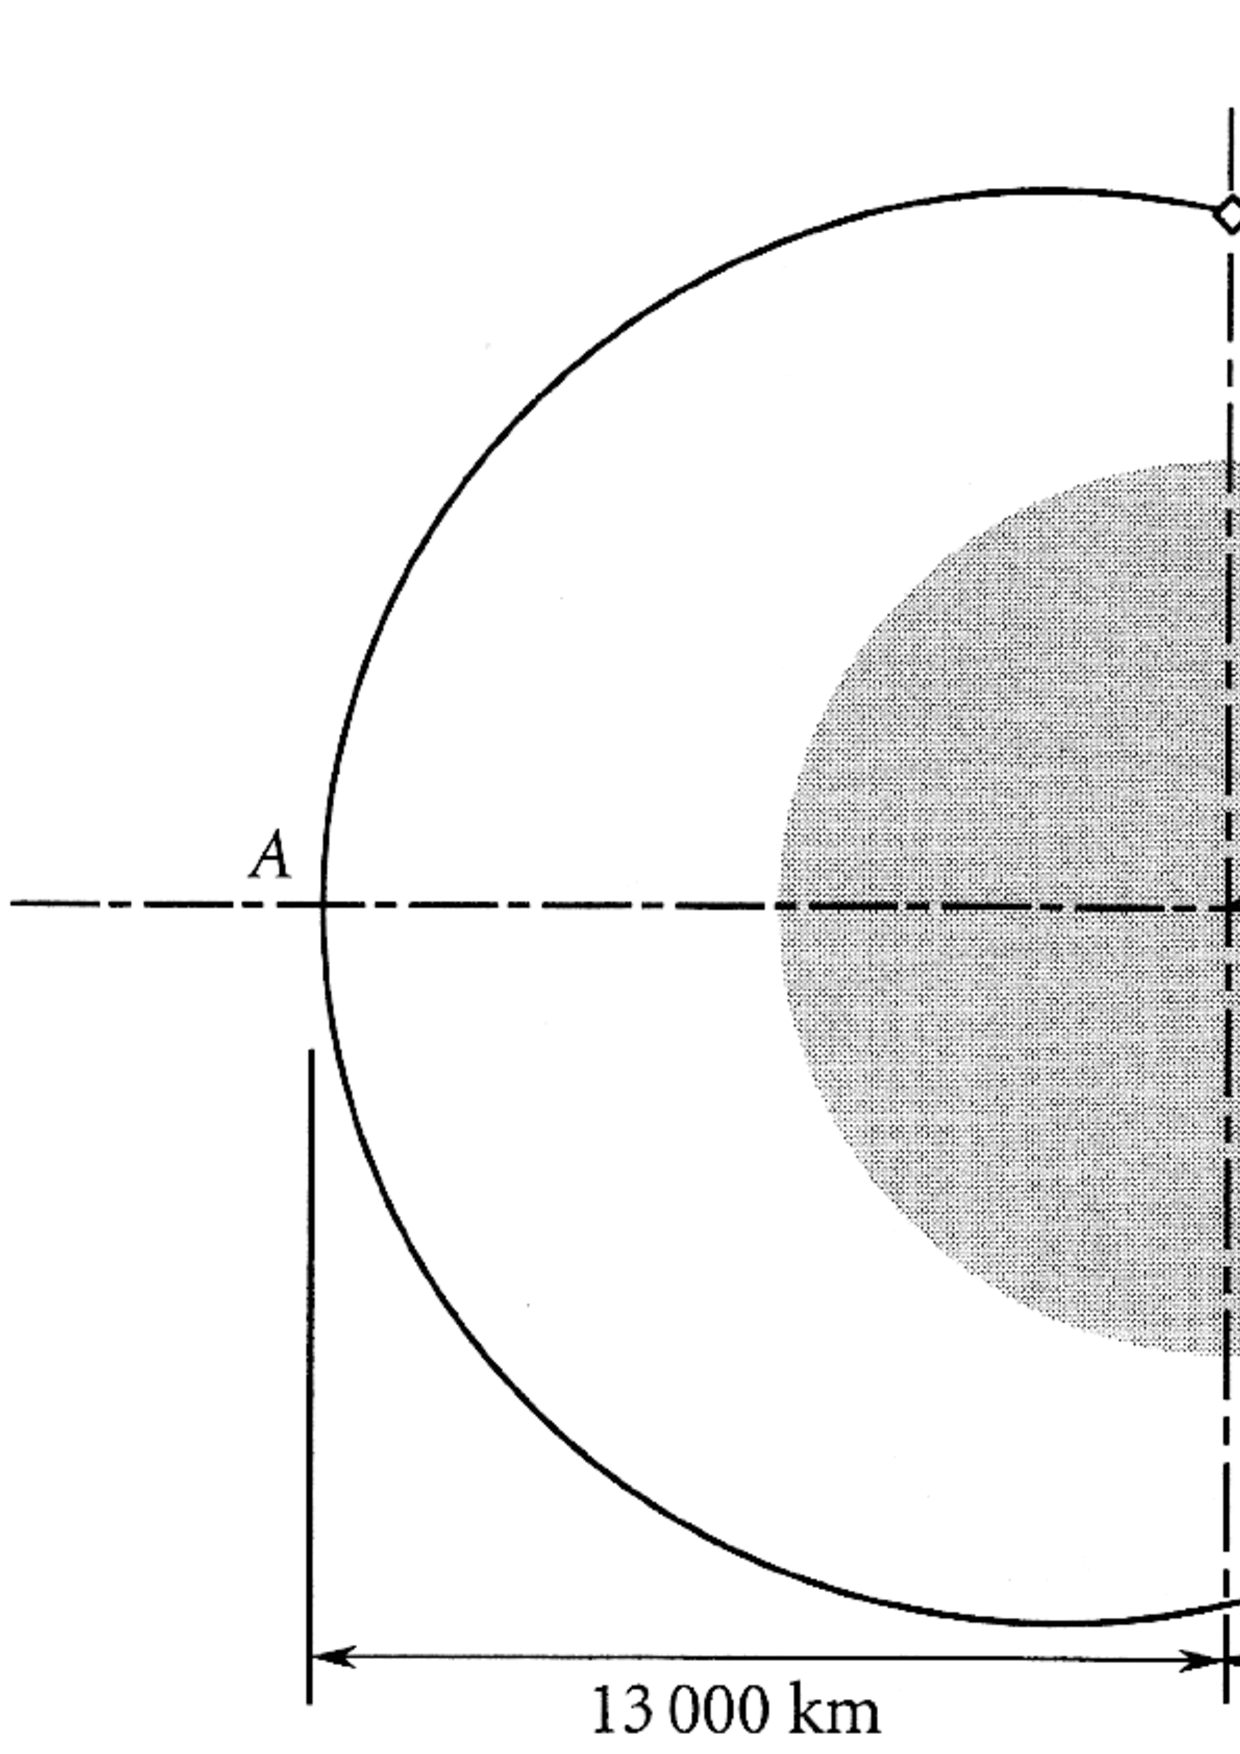
\includegraphics[width=\textwidth]{prob2.png}
    \end{figure*}
\end{prob}

\extrapage
\extrapage

\begin{prob}
The following problems should be easy. 
Do not spend large amounts of time here.
\begin{subprob}
\item Draw a picture to explain why Greenwich Sidereal Time is approximately \SI{100}{\degree} at \num{0000} UTC on 1 January each year.
    Recall that the Winter Solstice is in the third week of December annually.

\item Given the total energy of a circular orbit, show that the orbital speed is constant and given by \( v_{circ} = \sqrt{\frac{\mu}{r}}\).

\item The Molniya orbit is a highly eccentric orbit specifically designed such that the spacecraft spends the majority of time in the vicinity of apogee.

    \begin{subprob}

    \item How would you determine the velocity of the Molniya orbit  at \underline{perigee}?
    Assume you are given the semi-major axis, \( a \), and eccentricity, \( e\).
    Express your solution in terms of \( a \) and \( e\).
        \item Determine the inclination required such that the argument of perigee remains constant?
        \item At this inclination what is the rate of right ascnension of the ascending node?
    \end{subprob}
\end{subprob}
\end{prob}

\extrapage
\extrapage

\begin{prob}
    To prepare for anti-satellite avoidance, US Space Command will require every satellite operator to generate a plot of total \( \Delta V \) versus time of flight (TOF) for their satellite to increase its altitude by \SI{25}{\kilo\meter}. 
    Provide an algorithm to generate this plot assuming that the satellites are initially in a circular orbit and the final orbit is circular and in the same inclination as the initial orbit. 
    Furthermore, assume that the first maneuver will be a tangential burn, while the second maneuver will be non-tangential ( a so called \textbf{One Tangent Burn}).

    \begin{subprob}
    \item Write your algorithm.
        Please write neatly and legibly.
        Furthermore, your algorithm should be in a logical sequence. 

        \textbf{GIVEN:} \( r_i\) (initial radius of circular orbit) and \( \Delta \nu\) (change in true true anomaly along the transfer orbit) from \SIrange{0}{180}{\degree}.

        \textbf{FIND:} Total \( \Delta V\) and TOF (time of flight)
        
    \item Draw a vector diagram showing all three velocity vectors involved in the second burn and label them correctly.
        Include the change in flight path angle \( \Delta \gamma \) and firing angle \( \alpha \).
    \end{subprob} 
\end{prob}    

\extrapage
\extrapage

\begin{prob}
    Your first job involves a boss who is aware of the SEZ frame but claims ``it doesn't make any sense''.
    Your boss would instead like to use the \textbf{North West Zenith} reference frame because it makes more sense.

    \begin{subprob}
    \item Determine the rotation matrices to transform a vector from the \textbf{North West Zenith} reference frame to the \textbf{Earth Centered Inertial} reference frame.
    \item From a site located at \SI{30}{\degree} North latitude and \SI{90}{\degree} West longitude, the range vector to a satellite is :
        \begin{align*}
            \bar \rho_{NWZ} = - 7000 \hat N - 500 \hat W + 500 \hat Z \si{\kilo\meter}
        \end{align*}
        at \( GST = 0600\) hours.
        What is the \underline{ \( \hat k = \hat z \) component} of this vector, \( \bar \rho_{ECI}\), in the \textbf{Earth Centered Inertial} reference frame?
    \end{subprob}
\end{prob}

\extrapage
\extrapage

\end{document}
